\documentclass[11pt]{standalone}

\usepackage{ifthen}
\usepackage{tikz} 
\usetikzlibrary{shapes.misc}
\usetikzlibrary{arrows,arrows.meta}
\usetikzlibrary{calc,intersections, patterns, math}

\definecolor{pfeil}{RGB}{168,167,167}
\definecolor{petrol}{RGB}{0, 118, 136}
\definecolor{darkgoldenrod}{RGB}{184, 134, 11}
\colorlet{petrol-lighter}{petrol!40}
\colorlet{darkgoldenrod-lighter}{darkgoldenrod!40}

\begin{document}

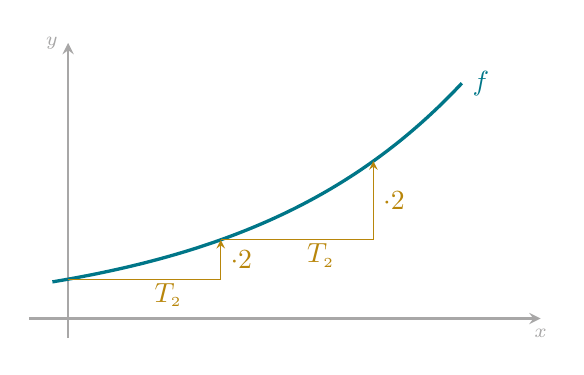
\begin{tikzpicture}[pfeil]

    % \draw[thick, fill=petrol!20, draw=petrol-lighter, rounded corners=2ex, opacity=0.5] (0,0) rectangle ++ (1.5,3.5);
    % \draw[thick, fill=darkgoldenrod!20, draw=darkgoldenrod-lighter, rounded corners=2ex, opacity=0.5] (5,0) rectangle ++ (1.5,3.5);

    \draw[thick, -stealth] (-0.5,0) -- (6,0) node[below]{$\scriptstyle x$};
	\draw[thick, -stealth] (0,-0.25) -- (0,3.5) node[left]{$\scriptstyle y$};
	
	\draw[very thick,domain=-0.2:5., smooth, samples=50, petrol] plot(\x,{0.5*1.43^(\x)}) node[right] {$f$};

    \draw[darkgoldenrod, -stealth] (0,0.5) -- node[below, yshift=0.7mm, xshift=3mm] {$T_{\scriptscriptstyle2}$} ++ (1.938,0) -- node[right] {$\cdot 2$} ++ (0,0.5);
    \draw[darkgoldenrod, -stealth] (1.938,1.) -- node[below, yshift=0.7mm, xshift=3mm] {$T_{\scriptscriptstyle2}$} ++ (1.938,0) -- node[right] {$\cdot 2$} ++ (0,1.);

\end{tikzpicture}

\end{document}
